\documentclass[12pt,letter]{article}

\usepackage{amsfonts}
\usepackage[english]{babel}
\usepackage[utf8]{inputenc}
\usepackage{mathtools}
\usepackage{amssymb}
\usepackage{graphicx}
\usepackage{gensymb}
\usepackage{tikz}
\usepackage{polynom}
\usepackage{amsthm}
\usepackage{arcs}
\usepackage{pifont}
\usepackage[colorinlistoftodos]{todonotes}
\usepackage{caption}
\usepackage{subfigure}
\newcommand*\rfrac[2]{{}^{#1}\!/_{#2}}

\newtheorem{definition}{Definition}
\newtheorem*{definition*}{Definition}

\DeclarePairedDelimiter\abs{\lvert}{\rvert}
\makeatletter
\let\oldabs\abs
\def\abs{\@ifstar{\oldabs}{\oldabs*}}%
% Absolute value symbol
\usepackage{setspace}
\doublespacing
\usepackage{fullpage}

\begin{document}

%Begin title block%
\title{Capsids and Stuff}
\author{Charles Zahara}
\maketitle
%End title block%

\section{Introduction}

% CITATION EXAMPE\cite[p 27]{Mannige:2009}

\paragraph{}
Mathematics has always been a beautiful field full of excitement and discovery. From purely theoretical considerations to strictly applied problems the mathematician is never without mental stimulus. Its inspirations are everywhere and one needs only to be willing to ask why and how to be able to find a fantastic problem to consider. Although the sciences sometimes lack a willingness to work together, Biology is a great realm within which to discover new questions. To find challenging mathematical problems within Biology, one does not need to be an applied mathematician with decades of experience in modeling. Nor does one need to have an extensive background in Biology and science. All that is required is to be willing to examine systems and be willing to ask questions.

The aim of this paper is to take the reader through the discovery of mathematical puzzles inspired by the physical world. Specifically these mathematical questions will come from the theory of spherical virus capsids. Two problems left unanswered by many of the works on the spherical virus capsids will be laid out and then multiple techniques for solving these problems will be detailed. Although this paper is centered around the mathematics of why icosahedral shells work, it aims to be readable by anyone without external materials, extensive background reading, or a 6' by 20' wall of white board to work out gaps in equations. This paper will ultimately demonstrate that unique problems in mathematics are everywhere and can often be solved with very basic tools if one is willing to apply some hard work and problem solving.

A secondary objective of this paper is to be an entertaining introduction to the theory of icosahedral symmetry of virus capsids. It is intended to be a type of tour guide through the development and arguments of this theory. As such, the paper begins with a review of both past and present work on virus capsids. First the pivotal works on the theory of symmetry in spherical virus capsids will be summarized. Then a few selections of the current work both biologists and mathematicians are performing in the field of virus capsids will be examined. Hopefully the reader will come away understanding not only the form and function of icosahedral capsids, but also the amazing, challenging, and ultimately fun mathematical problems that arise within Biology. 

\section{Background} %%%%% 1. Background

\paragraph{}
Viruses have been shaping human history for millennia. From smallpox and polio to the yearly strains of flu and common cold, every generation has battled against these tiny creatures. They have wiped out civilizations and continue to kill millions every year. As such the study of their form and function remains important.

\begin{definition*}[Virus]
Viruses are infectious agents composed of nucleic acid surrounded by a protein shell, called a capsid, and in some cases a membranous envelope. \normalfont{ \cite{Campbell:2002} }
\end{definition*}
While the above definition may make viruses seem like simple little organisms, they have a multitude of unique variations. Their nucleic acid genetic material may come in the form of DNA or RNA, depending on the virus, and be either single or double stranded. They can be rod shaped, roughly spherical, or in some cases rather complex in shape. Additionally, viruses are very effective organisms. They cannot replicate or reproduce themselves, but instead inject their genetic material into a host cell. The host cell is then taken over and forced to create copies of the virus genetic material and capsid proteins. Eventually, once it is filled to capacity, the host cell bursts open and the newly created capsids are expelled and proceed to a new host to repeat the process (See Figure \ref{fig:life_cycle}). \cite{Campbell:2002}

\begin{figure}[h]
	\caption{Viral life cycle}
	\centering
	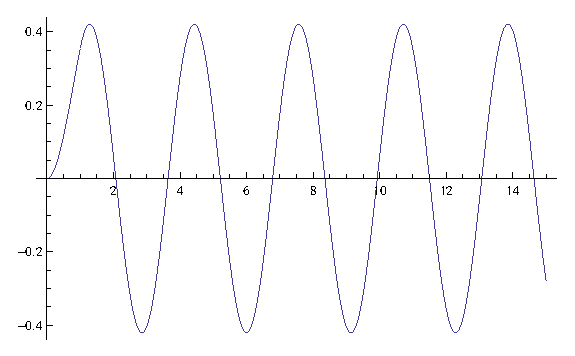
\includegraphics{place_holder.eps}
	\label{fig:life_cycle}
\end{figure}
	

The purpose of these capsid shells are to protect the virus genetic material as they move from host cell to host cell. This makes the capsid crucial in the infection process. It also means that understanding the structure and mechanics of the capsids may allow scientists to develop ways to disrupt their construction, thus eliminating the virus's ability to travel and infect new host cells. 

As stated previously, viruses come in a variety of shapes and sizes, defined by their capsid shells. Some are long tubes, similar to a straw, classified as helical viruses, others are roughly spherical, classified as icosahedral viruses, and others do not fall into either of the two previously mentioned categories and are classified as complex (See Figure \ref{fig:virus_types}). Spherical viruses are the focus of this paper. In the late 1950's and early 1960's it was suggested that spherical viruses capsids must conform to icosahedral symmetry \cite{Crick:1956}, \cite{Caspar:1962}. Although there are still many exceptions which continue to be examined, through decades of study and advances in microscope technology the theory that spherical capsids must have icosahedral symmetry has been confirmed both visually and computationally for most cases. What is often left unexplained in papers discussing spherical viruses is the mathematical reasoning behind the theory of their shape.

\begin{figure}[h]
	\caption{Viral life cycle}
	\centering
	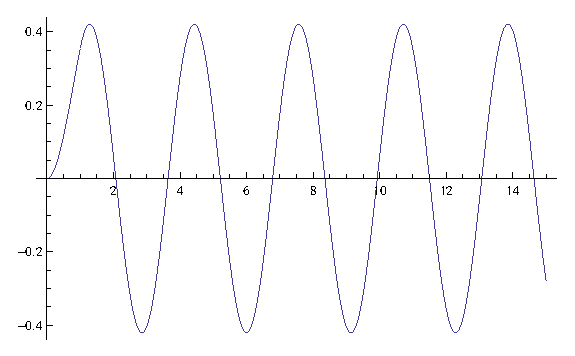
\includegraphics{place_holder.eps}
	\label{fig:virus_types}
\end{figure}

Before the history and theory are reviewed a few key definitions and their relationship are important.

\begin{definition*}[Capsid]
A viral capsid is a protein shell made up multiple copies of one, but in some cases a few, small proteins, which encloses and protects the viral genome.
\end{definition*}
\begin{definition*}[Capsomere]
A capsomere is a repeated symmetric building unit for the viral capsid. They are made up of multiple proteins.
\end{definition*}
\begin{definition*}[Protomer]
A promoter is a single protein unit of a capsomere.
\end{definition*}

The important note is that the protomeres are the smallest unit. They are single asymmetric proteins. Capsomeres are built up of multiple protomers in a symmetric fashion. There can be multiple differently shaped capsomeres made from the same protomer sub-unit. The Capsid is the final shell, made up of the capsomere building blocks.

\subsection{The History of Icosahedral Symmetry} %%%%% 2.1 History

\subsubsection{Initial Theories of Crick and Watson}
\paragraph{}
In 1956  F. H. Crick and J. D. Watson wrote a paper entitled "Structure of Small Viruses." In this paper they hypothesized that "a small virus contains identical sub-units, packed together in a regular manner" \cite[p 473]{Crick:1956}. While this was not an entirely new idea, Crick and Watson were the first to describe the specifics of the idea and to proclaim it as a feature of all small viruses. This hypothesis was based upon the fact that all plant viruses having been studied at the time were extremely "regular," meaning that for a particular virus each particle was similar, if not identical, in appearance. This belief was strengthened by the fact that viruses can form crystals, a feature only possible if each individual viral molecule is identical.

At the time of their writing, viruses had only been observed to follow the rod shape of the tobacco-mosaic virus (TMV), as studied by Tubingen and Berkley, or the spherical shape of the turnip yellow mosaic virus (TYMV), as studied by Markham. Indeed, more research had been done on the Tobacco Mosaic Virus than any spherical virus at the time and so many conjectures were made from these observations. For instance, the tobacco mosaic virus consists of 94\% protein and 6\% RNA \cite[p 473]{Crick:1956}. This suggests that proteins must be repeated as there is not enough RNA to code unique proteins in that ratio. Very early X-Ray work showed that the each TMV particle was made up of sub-units of some sort. More importantly, Crick and Watson were able to observe that the TMV particles had a screw like axis, which acted as a symmetry axis, thus placing each sub-unit in an identical environment as the rest.

It is unclear from their work whether or not the sub-units that Crick and Watson noticed on a TMV particle were capsomeres, the larger groups of proteins, or protomeres, the individual proteins themselves. It is most likely that due to limited tools they were making observations about capsomeres due to describing them as "small globular proteins" \cite[p 473]{Crick:1956}. Additionally, they spoke of the sub-unit being repeated in similar packing arrangements around the central axis \cite[p 474]{Crick:1956}. It was clearly shown later by Caspar and Klug that the capsomere is the repeated symmetrical unit, while the protomers are asymmetric units which aggregate to form the capsomeres. It is helpful to understand what Crick and Watson were observing on the TMV particles in order to understand why they made the conjectures they did about spherical virus.

Crick and Watson then extended their observations of the TMV particles to the less studied spherical viruses. It had been shown that TYMV and bushy stunt virus would crystalize into a unit cell that had the shape of a cube. This forces the individual virus particles to have cubic symmetry. Indeed, Crick and Watson were in communication with Caspar who had been able to clearly demonstrate the bushy stunt virus had cubic symmetry \cite[p 474]{Crick:1956}. 

Cubic symmetry relates to the rotational possibilities of the particle. It means that through the shell there are axes which one can rotate about 120\degree and the figure will end up in an identical position as it started. This axes are called 3-fold rotational axes. To see this in action, take a die and hold it by two opposing corners. Now rotate the die $\rfrac{1}{3}$ of a turn. Although the position of the numbers has changed, the die is in an identical position as it started. Thus this die, a cube, is an example of a figure with cubic symmetry.

While the virus particle can be rotated, the individual sub-units cannot be "flipped". This is due to the presence of asymmetric carbon atoms \cite[p 474]{Crick:1956}. This means there can be no reflective symmetry axes on the particle. For a visual representation of a figure rotational symmetry axes but no reflective symmetry axes see Figure ~\ref{fig:reflect}. Crick and Watson then examined all possible cubic point groups, which are listed in Table ~\ref{table:cubic_groups}. [Is it worth defining a point group?]

\begin{figure}[h]
	\caption{Symmetry examples. Use figures from Mannige}
	\centering
	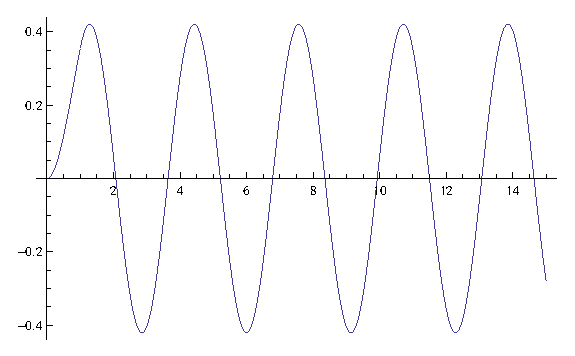
\includegraphics{place_holder.eps}
	\label{fig:reflect}
\end{figure}

\begin{figure}[h]
	\caption{Table of cubic point groups}
	\centering
	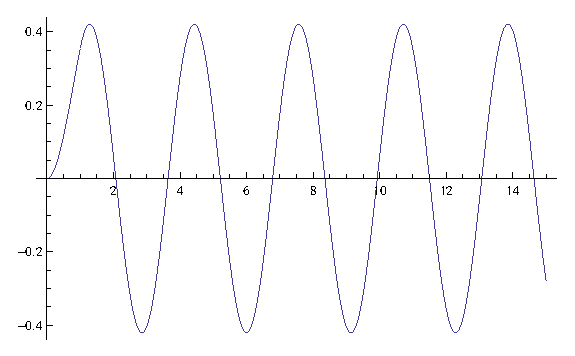
\includegraphics{place_holder.eps}
	\label{table:cubic_groups}
\end{figure}

They noticed that with each group, the number of possible asymmetric sub-units was a multiple of 12. For instance, with the 20 sided icosahedron, each side can be split into 3 asymmetric sub-units, thus creating a total of 60 which is of course a multiple of 12. Recall the reason they are concerned with the possible number of asymmetric units, not the number of faces, is because they wanted the smallest possible unit, and because the individual proteins were bound to be asymmetric simply due to their nature. This was their final, and ultimately erroneous conclusion, that the number of proteins in a viral shell will be a multiple of 12 \cite[p 475]{Crick:1956}.

It is important to note that their process was one of trying to apply a set of rules to the limited observations they had of both spherical and helical viruses. They were not trying to ask mathematical questions as to whether or not their results should be expected, but were instead simply trying to explain observed patters. This technique, of describing observations, was also the route taken by Caspar and Klug a few years later, only with a more accurate outcome.

\subsubsection{The Theory of Quasi-Equivalence}
\paragraph{}

D. L. D. Caspar and  A. Klug wrote many papers on the structure of viruses. Their most prominent work was done in 1962 in a paper entitled "Physical Principles in the Construction of Regular Viruses" \cite{Caspar:1962}. In this work they built upon the ideas and groundwork set forth by Crick and Watson, only with more scientific tools at their disposal. The results were to validate the general idea set forth by Crick and Watson, but to ultimately correct the theory and form what is still the basis of belief today.

Much of their paper repeats in greater detail the same concepts set forth by Crick and Watson. They why there may only be a limited number of types of proteins in any one capsid and why the number of ways to efficiently design a container using a large number of identical proteins is very limited. Only Caspar and Klug had more scientific evidence, largely due to the greater volume of research that had been performed by 1962. For instance, by studying the weight of the RNA within small viruses, and the average number of nucleotides required to make a protein, they were able to prove that there is only enough genetic material in small viruses to produce 2 or 3 proteins \cite[p 1]{Caspar:1962}. This proved that with small viruses the number of types of proteins in the capsids is limited to 1 or 2. Additionally, advances in X-ray diffraction and electron microscopy had definitively shown for multiple small viruses that they were indeed made up of repeated  identical sub-units \cite[p 2]{Caspar:1962}. What differed from Crick and Watson was the number of individual protomers possible in spherical viruses.

While Caspar and Klug ultimately disproved a flaw in Crick and Watson's theory for spherical viruses, it is worth noting that they also confirmed Crick and Watson's theory for helical ones.



\section{T-numbers}
\paragraph{}
Caspar and Klug claim that their T-number, $T = h^2 + hk + k^2$, defines the exact number of identical asymmetric protein sub-units found in a spherical capsid through the formula $P = 60T$. Recall this 60 is because the T number measure the number of triangular capsomers??? per side of the icosahedron and each capsomer is composed of 3 of the protein sub-unit. Since an icosahedron has 12 sides, we would have $3*12*T = 60T$ proteins per capsid. While their T-number has been confirmed as accurate through better microscopes (get type and shit), as mathematicians we should ask, was this expected? Will the T-number always work for integers h and k. If we use Caspar and Klug's approach of placing one corner of a triangular face of the icosahedron at $(0,0)$ on a P6 (what does this mean) grid, will the third corner always fall on another integer valued point of the grid? To answer these questions we will take 2 different approaches. One requires no mathematics beyond high-school, and the second only requires a bit of knowledge of linear algebra.

\subsection{The geometry approach}

\paragraph{}
The goal of this approach is to establish that if we are given a point $(h,k)$ as defined by Caspar and Klug (that is that the h-axis is the standard x-axis and the k-axis is a $60\degree$ rotation counter-clockwise of the h-axis) that the area of an equilateral triangle with a base from $(0,0)$ to $(h,k)$ will equal the area of an equilateral triangle with base length 1 times $T = h^2 + hk + k^2$. We will attempt to do this with no more than the skills of someone who has passed high school geometry. \\

First, recall that the area of an equilateral triangle is $A = \rfrac {\sqrt{3}} {4} \, b^2$ where $b$ is the length of any side of the triangle. If we did not know this formula off the top of our head, could we re-establish it? To begin, take an equilateral triangle with side length $b$ (figure). Draw a line from any corner to the midpoint of the opposing side. We now have 2 triangles. If we recall our triangle congruency theorems we can quickly see by the side-angle-side theorem that these triangles are congruent. This forces the angle we cut with our line to be bisected, and since we started with an equilateral triangle which has all angles equal to $60\degree$, we know the top angles are both $30\degree$ making our constructed line perpendicular to the base. \\

We now wish to find the length of our constructed line $l$. Thankfully the pythagorean theorem is all we need for this.
\begin{align*}
b^2 &= \left(\dfrac{b} {2}\right)^2 + l^2 \\
l^2 &= b^2 - \dfrac{b^2} {4} \\
l^2 &= \dfrac{3} {4} \, b^2 \\
l &= \sqrt{\dfrac{3} {4} \, b^2} \\
l &= \dfrac{\sqrt{3}} {2} \, b
\end{align*}
Thus using our standard triangle area formula of $A = \rfrac{1} {2} \, base * height$ we get
\begin{align*}
A &= \dfrac{1} {2} \, b * \dfrac{\sqrt{3}} {2} \, b \\
A &= \dfrac{\sqrt{3}} {4} \, b^2
\end{align*} \\

Recall our goal of establishing that the area of an equilateral triangle with a base from $(0,0)$ to $(h,k)$ will equal the area of an equilateral triangle with base length 1 times $T = h^2 + hk + k^2$. Consider the triangle created by drawing lines between $(0,0), \; (h,k) \; \text{and} \; (h,0)$. We know 2 of the side lengths and wish to find side length b. Applying our previous work, we know that the exterior angle at point $(h,0)$ is $60\degree$, so if we drop a line down from point $(h,k)$ perpendicular to our t-axis, we obtain a triangle we have already worked with and know the dimensions of. Since it is $k$ units from $(h,0)$ to $(h,k)$ we know the perpendicular we just drew has length $\rfrac{\sqrt{3}} {2} \, b$ and the final leg of the triangle is $\rfrac 1 2 \, b$.

\section{What do trapezoids have to do with it?}
This entire section is wrong. You fucked up cause you're fucking retarded.

\paragraph{}
One constant and often unexplained attribute within works discussing icosahedral virus capsids is the authors' choice of subunit shape. Almost always the subunit is represented by a trapezoid with little to no explanation of why. If we recap what we know so far:
\begin{enumerate}
	\item Capsids are made up of pentamers and hexamers
	\item Hexamers are capable of existing in a "flat" state
	\item Three subunits need to make up an equilateral triangle
\end{enumerate}
Given these conditions, especially point (3), we may simply guess that trapezoids are used because every equilateral triangle can be split into three identical (right word?) isosceles trapezoids (See INSERT figure). 

But then we must ask why not some other shape that also has this property. For instance, equilateral triangles can also be split into three identical isosceles triangles or three identical right kites. To demonstrate, extend angle bisectors from each corner of an equilateral triangle until they meet in its interior. The result is that we have split the initial equilateral triangle into three identical isosceles triangles. Or we could create perpendicular bisectors on each side of an equilateral triangle and extend them within the interior of the triangle until they meet. This will result in the triangle being split into three identical right kites. (see INSERT figure) So again we must ask, why are trapezoids the standard subunit shape if other shapes will also meet our criteria of being able to fit perfectly inside an equilateral triangle?

Upon examination of shaded and deciphered images of real world icosahedral capsids we can see that the choice of trapezoid is simply due to their real world occurrence. (See [INSERT] capsid images) This was mentioned as early as (get date) by (get guy from mannige thesis)But this is a very interesting phenomenon. As pointed out by 



\bibliographystyle{IEEEtran}
\bibliography{Capsid_Cites}



\end{document}